\begin{section}{Metodologia}
O servidor, por ser o elemento chave na consolida��o do projeto, deve ser o 
m�dulo a ser prioritariamente configurado, a fim de ser preparado para atender
�s devidas requisi��es, bem como executar qualquer tipo de aplica��o solicitada.
Sendo assim, a instala��o da plataforma �ngstr\"{o}m foi tomada como o primeiro
passo. �ngstr\"{o}m~\cite{angstrom} � um sistema operacional, baseado em Linux,
preparado exclusivamente para plataformas embarcadas, sendo o padr�o para a 
pr�pria BeagleBone. 
As depend�ncias a serem instaladas s�o listadas na Lista~\ref{lst:dependences}.

\begin{lstlisting}[language=bash, caption={Pre-instala��o de depend�ncias no
servidor}, label={lst:dependences}]
# eSpeak dependences
libespeak-dev libportaudio2 libportaudio-dev

# Julius dependences
libasound2 libasound2-dev

# LAMP dependences
apache2 libapache2-mod-fastcgi
php5 libapache2-mod-php5 php5-mcrypt # PHP
mysql-server libapache2-mod-auth-mysql php5-mysql # MySQL
phpmyadmin
libmysqlclient-dev # C
libmysqlcppconn7 libmysqlcppconn-dev # C++
\end{lstlisting}

% http://eda.eme.ro/handle/10598/28187
Em~\cite{cassio14}, o Julius foi configurado para funcionar em modo servidor
atrav�s da op��o nativa ``-adinnet'' (A/D \textit{Input from Network}, convers�o 
A/D com entrada pela rede). Isso permite que o Julius receba amostras de �udio
via \textit{streaming} atrav�s de uma comunica��o com um cliente gen�rico via
\textit{socket}. O c�digo foi alterado para que o resultado gerado pelo Julius,
tamb�m conhecido como senten�a, seja retornado ao cliente atrav�s desse mesmo
\textit{socket}.

\begin{minipage}[t]{.50\textwidth}
\begin{lstlisting}
<s> aumentar volume </s>
<s> diminuir volume </s>
<s> canal mais </s>
<s> canal menos </s>
<s> canal <n�mero> </s>
<s> ligar televis�o </s>
<s> desligar televis�o </s>
<s> cadastrar controle </s>
...
\end{lstlisting}
\end{minipage}
\begin{minipage}[t]{.50\textwidth}
\begin{lstlisting}
aumentar	a u~ m e~  t a X  
diminuir	dZ i~ m i~ n u j X  
televis�o	t e l e v i z a~ w~   
volume		v o l u~ m i  
canal		k a n a w  
um			u~   
dois		d o j s  
tr�s		t r e j s
...
\end{lstlisting}
\end{minipage}

% http://stackoverflow.com/questions/2661129/espeak-sapi-dll-usage-on-windows

\begin{figure}[!h]
	\centering
	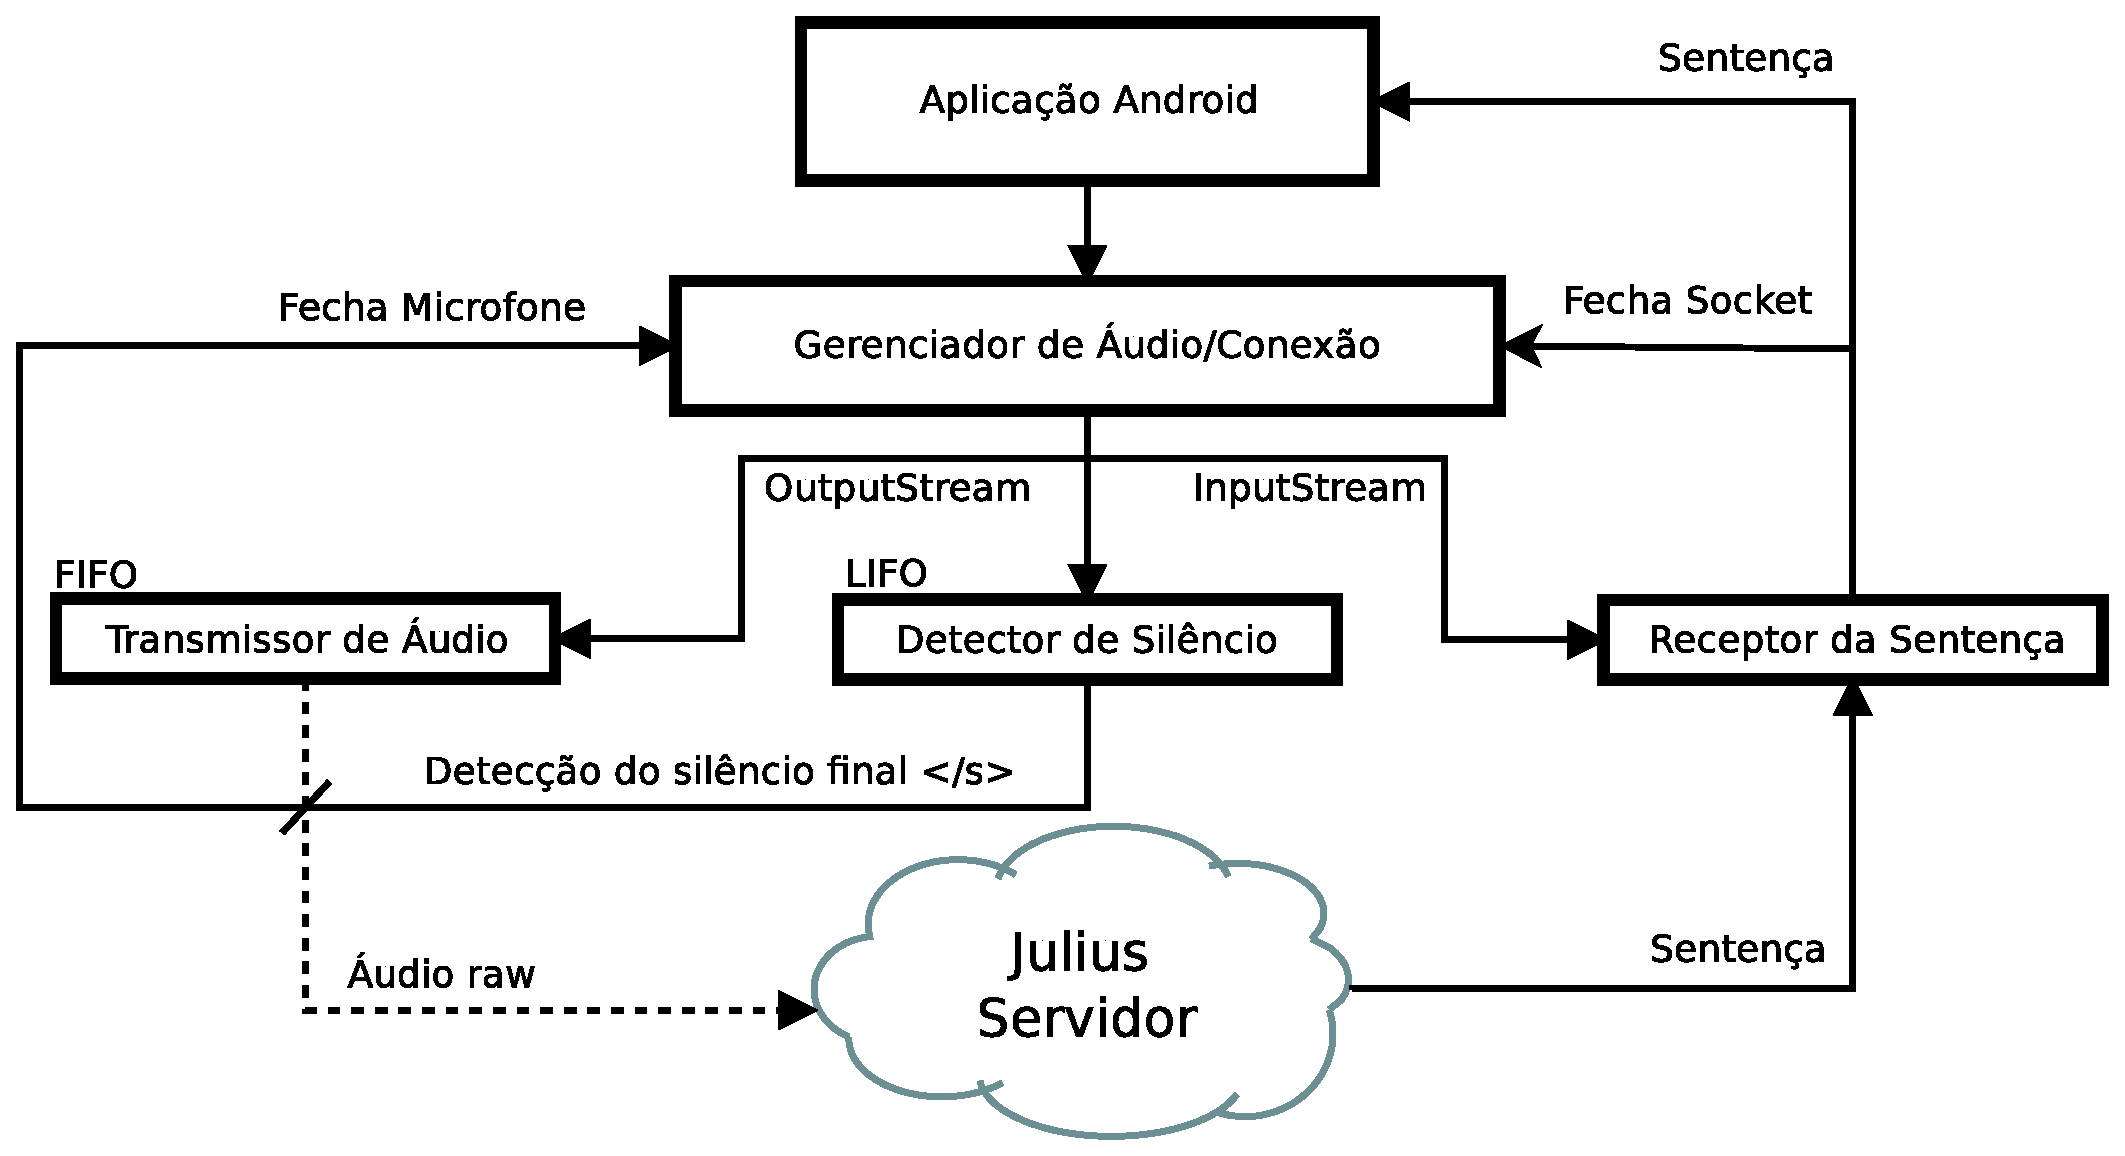
\includegraphics[width=.85\textwidth]{Figures/csr}
	\caption{Esquem�tico do Cliente LaPS CSR.}
	\label{fig:lapscsr_sch}
\end{figure}

\end{section}
%%% EOF %%%
